
\refstepcounter{Exercise}
\clearpage\subsection*{\theExercise URLを使ってCGIに情報を\ruby{渡}{わた}す}
\addtocounter{Exercise}{-1}\refstepcounter{Exercise}\label{E:URL}

% \clearpage\subsection*{URLを使ってCGIに情報を\ruby{渡}{わた}す}
考え方

CGIのプログラムに情報を渡すことができればより便利なプログラムが作れます。ここでは\ruby{単純}{たんじゅん}なURLを用いた方法を使います。URLに\ruby{埋}{う}め込まれた情報はクエリストリングと呼ばれます。クエリストリングはまずウェブサーバへ送られ、ウェブサーバがCGIプログラムへクエリストリングを渡します。これによりCGIプログラムはURLに埋め込まれた情報を扱うことができます。


\bigskip

まずは、ブラウザを開いて、

localhost:3000/cgi-bin/querystring.hsp?msg=helloworld

を入力してみましょう。

%
%ぶらうざで開いた画面
%helloworldと表示されている
%koyaman
%September 20, 2019 2:49 AM


画面にhelloworldと表示されたと思います。



\centering
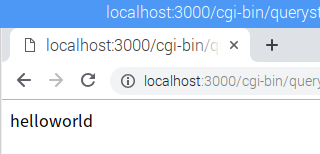
\includegraphics[width=0.8\textwidth]{text07-img/ome7-img053.png}
\flushleft

localhost:3000/cgi-bin/querystring.hsp?msg=goodbye

に変更してみてください。

%
%ぶらうざで開いた画面
%goodbyeと表示されている
%koyaman
%September 20, 2019 2:49 AM


次はgoodbyeと表示されたと思います。


\centering
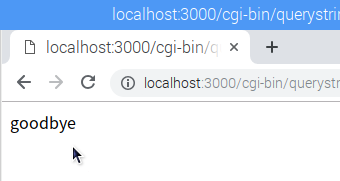
\includegraphics[width=0.8\textwidth]{text07-img/ome7-img054.png}
\flushleft

\clearpage

このようにURLに情報を埋め込んでおくことでCGIのプログラムはこれを受け取り処理をすることができます。URLに埋め込まれた情報はクエリストリングと呼ばれます。この情報はまずウェブサーバが受け取ります。ウェブサーバは少し\ruby{処理}{しょり}をしてCGIプログラムへ渡します。

クエリストリングはURLの最後に?をつけて始めます。

クエリストリングの形は

名前=値

のようになっています。この例では

msg=helloworld

msg=goodbye

などとなっています。これはmsgという名前の値はhelloworld,
goodbyeであることを意味します。HSPの変数と同じような感じです。

次にCGIプログラムでどのようにクエリストリングを扱っているのか見てみましょう。


\bigskip

プログラム解説





\begin{table}[htbp]
    \centering
    % \caption{文字タイプ表}
    \begin{tabular}{|l|}
        \hline
        
        1. \#include {\textquotedbl}hsp3cl.as{\textquotedbl}\\ 
        2. \#include {\textquotedbl}cgi.as{\textquotedbl}\\
        3. mes {\textquotedbl}Content-type: text/html{\textbackslash}n{\textquotedbl}\\
        4. mes {\textquotedbl}{\textless}html{\textgreater}{\textless}head{\textgreater}{\textless}meta charset={\textbackslash}{\textquotedbl}utf-8{\textbackslash}{\textquotedbl}{\textgreater}{\textless}/head{\textgreater}{\textless}body{\textgreater}{\textquotedbl}\\
        5. getqueryval {\textquotedbl}msg{\textquotedbl}, q\\
        6. mes q\\
        7. mes {\textquotedbl}{\textless}/body{\textgreater}{\textless}/html{\textgreater}{\textquotedbl}\\
        8. end
        
        
        \\\hline
    \end{tabular}
\end{table}




\bigskip


\bigskip

5行目の

getqueryval “msg”, q

はクエリストリング内の名前が”msg”に対応する値を変数qに入れています。

localhost:3000/cgi-bin/querystring.hsp?msg=helloworld

というURLがあった場合、

変数qにはhelloworldが文字列として入ります。

6行目で表示をしています。

このように\ruby{簡単}{かんたん}にプログラムでクエリストリングを受け取ることができます。クエリストリングが使えると、{\textless}form{\textgreater}{\textless}/form{\textgreater}を使ってCGIに処理を\ruby{依頼}{いらい}できたり、CGIの処理をより高度にすることができます。次の例では、クエリストリングを使ってLEDを点灯消灯します。

ほとんどのウェブサイトは検索をするさいにURLに検索ワードを埋め込んでいます。


\bigskip

\refstepcounter{Question}\theQuestion 画面に”ありがとう”と表示させよう。
% 問題7-11  
% 画面に”ありがとう”と表示させよう。